\documentclass{article}
\usepackage[margin=1in]{geometry}
\usepackage{problemset}
\showsolntrue

% Custom commands
\newcommand{\R}{\mathbb{R}}
\newcommand{\X}{\mathcal{X}}
\newcommand{\Y}{\mathcal{Y}}
\newcommand{\E}{\mathbb{E}}
\newcommand{\V}{\text{Var}}
\renewcommand{\P}{\mathbb{P}}
\newcommand{\x}{\mathbf{x}}
\newcommand{\h}{\mathbf{h}}
\newcommand{\y}{\mathbf{y}}
\newcommand{\w}{\mathbf{w}}
\newcommand{\p}{\mathbf{p}}

\begin{document}

\pstitle{%
    COGS 181%
}{
    Homework 5%
}[due Thursday, March 5 at 11:59PM]

\textbf{Instructions:} Answer the questions below, attach your code, and insert figures to create a PDF file; submit your file via Gradescope. You may look up the information on the Internet, but you must write the final homework solutions by yourself.

\textbf{Late Policy:} 5\% of the total points will be deducted on the first day past due. Every 10\% of the total points will be deducted for every extra day past due.

\textbf{System Setup:} You can install Anaconda to setup the Jupyter Notebook environment. Most packages have been already installed in Anaconda. If some package is not installed, you can use \texttt{pip} to install the missing package, that is, just type \texttt{pip install PACKAGE\_NAME} in the terminal.

\vspace{1em}

\begin{probset}
% --- Problem 1 ---
\begin{prob}[\textbf{(12 points) Conceptual Questions}]
    \begin{subprobset}
    \begin{subprob}
        \textbf{(3 points)} Given an n-character sequence, we want to predict which character would be the n + 1 th character in the sequence. For example, our input is "neura" (which is a 5-character sequence) and we have to predict what would be the 6th character. 
        
        Which neural network architecture would be \textbf{most} suitable to complete this task?
        \begin{enumerate}[label=\Alph*.]
            \item Fully-Connected Feed-Forward Network
            \item Convolutional Neural Network
            \item Recurrent Neural Network
            \item Hopfield Network
        \end{enumerate}

        \begin{soln}
            C. Recurrent Neural Network
        \end{soln}
    \end{subprob}

    \begin{subprob}
        \textbf{(3 points)} What is the technical difference between the vanilla backpropagation algorithm and the backpropagation through time (BPTT) algorithm? Choose \textbf{one}.
        \begin{enumerate}[label=\Alph*.]
            \item Unlike backprop, in BPTT we sum up gradients for corresponding weight \textbf{across all} time steps.
            \item Unlike backprop, in BPTT we multiply gradients for corresponding weight \textbf{across all} time steps.
            \item Unlike backprop, in BPTT we take the maximum gradient for corresponding weight \textbf{across all} time steps.
        \end{enumerate}

        \begin{soln}
            A. Unlike backprop, in BPTT we sum up gradients for corresponding weight \textbf{across all} time steps.
        \end{soln}
    \end{subprob}

    \newpage

    \begin{subprob}
        \textbf{(3 points)} What is the main idea behind self-attention in Transformers?
        \begin{enumerate}[label=\Alph*.]
            \item To allow the network to attend to different parts of the input sequence with varying degrees of importance.
            \item To train the network to classify the input sequence into different categories based on their features.
            \item To reduce the computational complexity of the network by learning a compact representation of the input sequence.
            \item To enable the network to learn multiple representations of the same input sequence simultaneously.
        \end{enumerate}

        \begin{soln}
            A. To allow the network to attend to different parts of the input sequence with varying degrees of importance.
        \end{soln}
    \end{subprob}

    \begin{subprob}
        \textbf{(3 points)} Which of the following statements is true about the differences between Recurrent Neural Networks (RNNs) and Transformers?

        \begin{enumerate}[label=\Alph*.]
            \item RNNs can handle variable-length inputs more efficiently than Transformers.
            \item Transformers have a better ability to capture long-term dependencies than RNNs due to their self-attention mechanism.
            \item Both RNNs and Transformers can handle sequential data, but RNNs are better suited for tasks that require online processing.
            \item Transformers are more computationally efficient than RNNs and can handle longer input sequences.
        \end{enumerate}

        \begin{soln}
            B. Transformers have a better ability to capture long-term dependencies than RNNs due to their self-attention mechanism.
        \end{soln}
    \end{subprob}
    \end{subprobset}
\end{prob}

\newpage

% --- Problem 2 ---
\begin{prob}[\textbf{(20 points) Recurrent Neural Network}]
    In this section, we will use a recurrent neural network (RNN) to process input sequence $\newline \x_t = \{\x_1, \x_2, \ldots, \x_{T-1}, \x_T\}$ where $\x_t \in \R^m$ and predict output sequence $\y_t = \{\y_1, \y_2, \ldots, \y_{T-1}, \y_T\}$ where $\y_t \in \R^n$. The RNN's structure is shown below:

    \begin{center}
        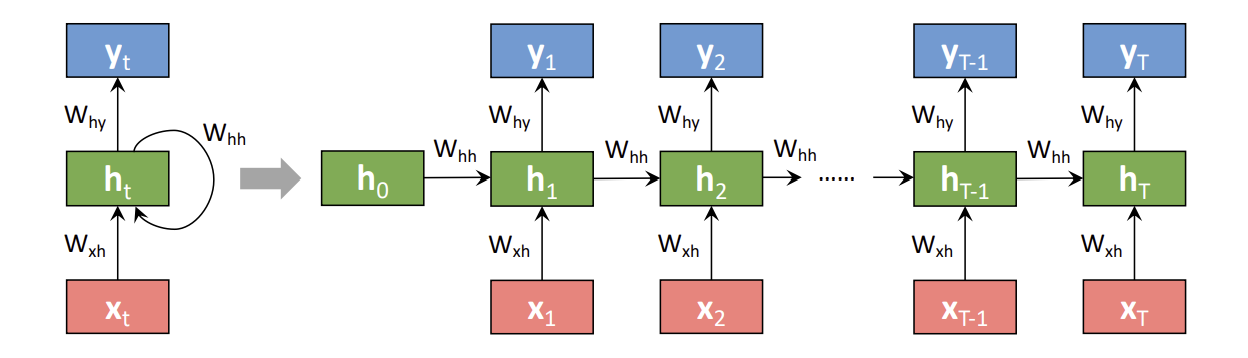
\includegraphics[width=\textwidth]{Images/2.png}
    \end{center}

    The left part of the figure is a common illustration of RNN, which includes three parameters $W_{xh} \in \R^{m \times l}$, $W_{hh} \in \R^{l \times l}$, $W_{hy} \in \R^{l \times n}$ and a hidden state $\h_t \in \R^l$. It includes two steps:

    \begin{enumerate}
        \item Compute hidden state: $\h_t = \text{ReLU}(W_{xh} \x_t + W_{hh} \h_{t-1})$.
        \item Predict the output: $\y_t = W_{hy} \h_t$.
    \end{enumerate}

    The right part of the figure shows the “unrolled” version of the RNN, which is the real computing path of the network:

    \begin{enumerate}
        \item In the initial stage, you have the initial hidden state $\h_0$.
        \item Then, after feeding the first input $\x_1$ of the sequence, RNN will compute the current hidden state $\h_1 = \text{ReLU}(W_{xh} \x_1 + W_{hh} \h_0)$ where $\text{ReLU}(z) = \max(0, z)$.
        \item Afterwards, the RNN will compute the output $\y_1 = W_{hy} \h_1$ and enter next round.
        \item In the next round, the RNN will generate hidden state $\h_2 = \text{ReLU}(W_{xh} \x_2 + W_{hh} \h_1)$ and the output $\y_2 = W_{hy} \h_2$. Eventually, the RNN will compute for $T$ rounds and predict the whole output sequence $\{\y_t\} = \{\y_1, \y_2, \ldots, \y_{T-1}, \y_T\}$.
    \end{enumerate}

    Assume $m = 1$, $n = 1$, $l = 2$. We are given the initial hidden state $\h_0 = \begin{bmatrix} 1 \\ 1 \end{bmatrix}$, the parameters $W_{hh} = \begin{bmatrix} 1 & -1 \\ 2 & -3 \end{bmatrix}$, $W_{xh} = \begin{bmatrix} 1 \\ -1 \end{bmatrix}$ and $W_{hy} = \begin{bmatrix} -2 & 3 \end{bmatrix}$, and an input sequence $\{ \x_1 = 3, \x_2 = 5 \}$.

    \textbf{Please calculate the values of the output $\y_1$ and $\y_2$ using the unrolled version of the RNN.}

    \begin{soln}
        \begin{align*}
            \h_1 &= \text{ReLU}(W_{xh} \x_1 + W_{hh} \h_0) = \text{ReLU}\left(\begin{bmatrix} 1 \\ -1 \end{bmatrix} (3) + \begin{bmatrix} 1 & -1 \\ 2 & -3 \end{bmatrix} \begin{bmatrix} 1 \\ 1 \end{bmatrix}\right) = \begin{bmatrix} 3 \\ 0 \end{bmatrix} \\
            \y_1 &= W_{hy} \h_1 = \begin{bmatrix} -2 & 3 \end{bmatrix} \begin{bmatrix} 3 \\ 0 \end{bmatrix} = -2 \cdot 3 + 3 \cdot 0 = -6 \\
            \h_2 &= \text{ReLU}(W_{xh} \x_2 + W_{hh} \h_1) = \text{ReLU}\left(\begin{bmatrix} 1 \\ -1 \end{bmatrix} (5) + \begin{bmatrix} 1 & -1 \\ 2 & -3 \end{bmatrix} \begin{bmatrix} 3 \\ 0 \end{bmatrix}\right) = \begin{bmatrix} 8 \\ 1 \end{bmatrix} \\
            \y_2 &= W_{hy} \h_2 = \begin{bmatrix} -2 & 3 \end{bmatrix} \begin{bmatrix} 8 \\ 1 \end{bmatrix} = -2 \cdot 8 + 3 \cdot 1 = -16 + 3 = -13
        \end{align*}
    \end{soln}
\end{prob}

\newpage

% --- Problem 3 ---
\begin{prob}[\textbf{(22 points) Hopfield Network}]
    In this homework problem, we will write a program to “train” and simulate a Hopfield network that memorizes 1-D vector patterns.

    \textbf{Training (Constructing Weights)}

    Instead of “training” a Hopfield network in the sense that you're used to, the weight matrix in Hopfield networks can be calculated directly using a formula provided in the original paper. Suppose we have $N$ nodes and $M$ states and (here $M = 2$) is the number of states to calculate $W$ and can be retrieved by using $W$. For each possible state $V^s$, $s = 1, \ldots, M$, the value of elements in $V^s$ is either -1 or +1. We can compute the weight matrix using:
    \begin{align}
        W_{ij} = \frac{1}{N} \sum_{s=1}^{M} V^s_i V^s_j, \quad \text{ if } i \neq j
    \end{align}
    And the diagonal values of the weight matrix are all zero, i.e. $w_{ii} = 0$.

    \textbf{Probing Pattern}

    Given an unknown pattern $V_{new}$, you will initialize the Hopfield network output nodes at time $t$, $U_i(t)$ as follows:
    \begin{align}
        U_i(0) = V^{new}_i, \quad i = 1, \ldots, n
    \end{align}
    
    \textbf{Dynamic Evolution}

    The inference procedure is very similar to what you have done in perceptron. Iterate until convergence:
    \begin{align}
        U_i(t + 1) = f_h\left(\sum_{j=1,j\neq i}^{N} W_{ji} U_j (t)\right)
    \end{align}
    $f_h(x)$ is a hard-limiting non-linearity function, where $f_h(x) = +1$ when $x \geq 0$ and $f_h(x) = -1$ when $x < 0$.

    In this step, you need to determine an order for updating the nodes \textbf{asynchronously which means all units should be updated in sequential at time $t$}. Typically we use a random visiting sequence (e.g. for a 4-node network, an order can be 2,3,4,1,2,3,4,1,2,3,4,1$\ldots$). 
    
    The stopping criterion is when the outputs from the node remain unchanged. This means that if you go through $N$ consecutive neurons without changing any of their values, then you're at a fixed point so you can stop.

    \textbf{Hint:}
    \begin{itemize}
        \item At time $t$, $U$ should be updated $N$ times.
        \item LastU stores the value of $U$ before update and is only used to compare with $U$ after $N$-times update to stop the evolution.
    \end{itemize}

    \textbf{Your Tasks}

    Write code to build a 5-node Hopfield Network which can converge to the following two states respectively following below procedure:
    \begin{itemize}
        \item (-1, +1, +1, -1, +1)
        \item (+1, -1, +1, -1, +1)
    \end{itemize}
    
    Please modularize your code to explicitly perform the three steps (Training, Probing Pattern, Dynamic Evolution).
    For the Probing Pattern step, please use the initial input state vector $V^{new}$ = 
    \begin{itemize}
        \item (+1, +1, +1, +1, +1)
    \end{itemize}

    For the Dynamic Evolution step, please try two different node visiting orders respectively starting from $V^{new}$:
    \begin{itemize}
        \item $(3, 1, 5, 2, 4, 3, 1, 5, 2, 4...)$
        \item $(2, 4, 3, 5, 1, 2, 4, 3, 5, 1...)$
    \end{itemize}

    Download the skeleton code \texttt{hw5-hopfield.ipynb} from the course website. Complete the skeleton code. In order to get full marks, your report should include:

    \begin{itemize}
        \item Attach the code,
        \item Log the node updating history at each iteration (print out each $U_i(t+ 1)$ you get during evolution).
        \item Show the matching between the retrieved pattern (the final fixed-point state your network converges to) and the evolving sequence.
    \end{itemize}


    \begin{soln}
        Code is attached at the end along with the logs.

        Starting from $V^{new} = (+1, +1, +1, +1, +1)$
        \begin{itemize}
            \item Order $(3, 1, 5, 2, 4, \ldots)$: converges to $(-1, +1, +1, -1, +1)$.
            \item Order $(2, 4, 3, 5, 1, \ldots)$: converges to $(+1, -1, +1, -1, +1)$.
        \end{itemize}
        Both fixed points match the two stored patterns.
    \end{soln}
\end{prob}

\newpage

% --- Problem 4 ---
\begin{prob}[\textbf{(21 points) Hopfield Network for TSP}]
    In this problem, we will use a Hopfield Network to solve a small instance of the Traveling Salesman Problem (TSP). The goal of TSP is to find a shortest possible tour that visits each city exactly once and returns to the starting city.

    \textbf{Problem Setup}

    We will solve a TSP that visits 6 cities: San Diego, Los Angeles, Boston, New York, Chicago, Seattle. The reference latitude/longitude coordinates for the cities are given below:
    \begin{itemize}
        \item \texttt{San Diego (-117.1611, 32.7157)}
        \item \texttt{Los Angeles (-118.2437, 34.0522)}
        \item \texttt{Chicago ( -87.6298, 41.8781)}
        \item \texttt{New York ( -74.0060, 40.7128)}
        \item \texttt{Boston ( -71.0589, 42.3601)}
        \item \texttt{Seattle (-122.3321, 47.6062)}
    \end{itemize}

    \textbf{What to Implement}

    \begin{enumerate}
        \item \textbf{Distance Matrix}
        Construct a distance matrix $D \in \R^{N \times N}$ from the city coordinates (e.g., Euclidean distance on latitude/longitude). You may normalize distances (recommended) to stabilize optimization.
        \item \textbf{Hopfield Formulation for TSP}
        Implement the Hopfield network with an iterative update rule (continuous or discrete) that drives the neuron activations toward a matrix $V \in [0, 1]^{N \times N}$, where $V_{i,j}$ encodes assigning city $i$ to tour position $j$.
        \item \textbf{Decoding a Tour}
        Decode the tour from $V$ after training. A valid tour must contain each city exactly once.
        \item \textbf{Visualization (Required)}
        Your submission must show:
        \begin{itemize}
            \item \textbf{Route Map}: the evolving/final tour on a 2D map (lon/lat scatter + connections)
            \item \textbf{V Matrix Heatmap}: activations as a heatmap [city $\times$ position], including all 6 cities.
            \item \textbf{Energy Curve}: energy vs. iteration steps (should generally decrease)
        \end{itemize}
    \end{enumerate}

    No skeleton code is provided for this task. You may refer to the \href{https://piazza.com/class_profile/get_resource/mk2x4slusi46uh/mlu42jq4m762nt}{demo notebook} on the course website. You may use it as a starting point, but note that it has a bug (the V matrix for the Los Angeles row is all 0). \textbf{You are encouraged to use coding assistants (e.g., Claude Sonnet, Cursor, Copilot) to support vibe coding and debugging for this problem.}

    Your report should include the code, and the visualization results mentioned above

    \begin{soln}
        Code is attached at the end. The decoded tour is $(3, 4, 0, 5, 2, 1)$.
        \begin{center}
            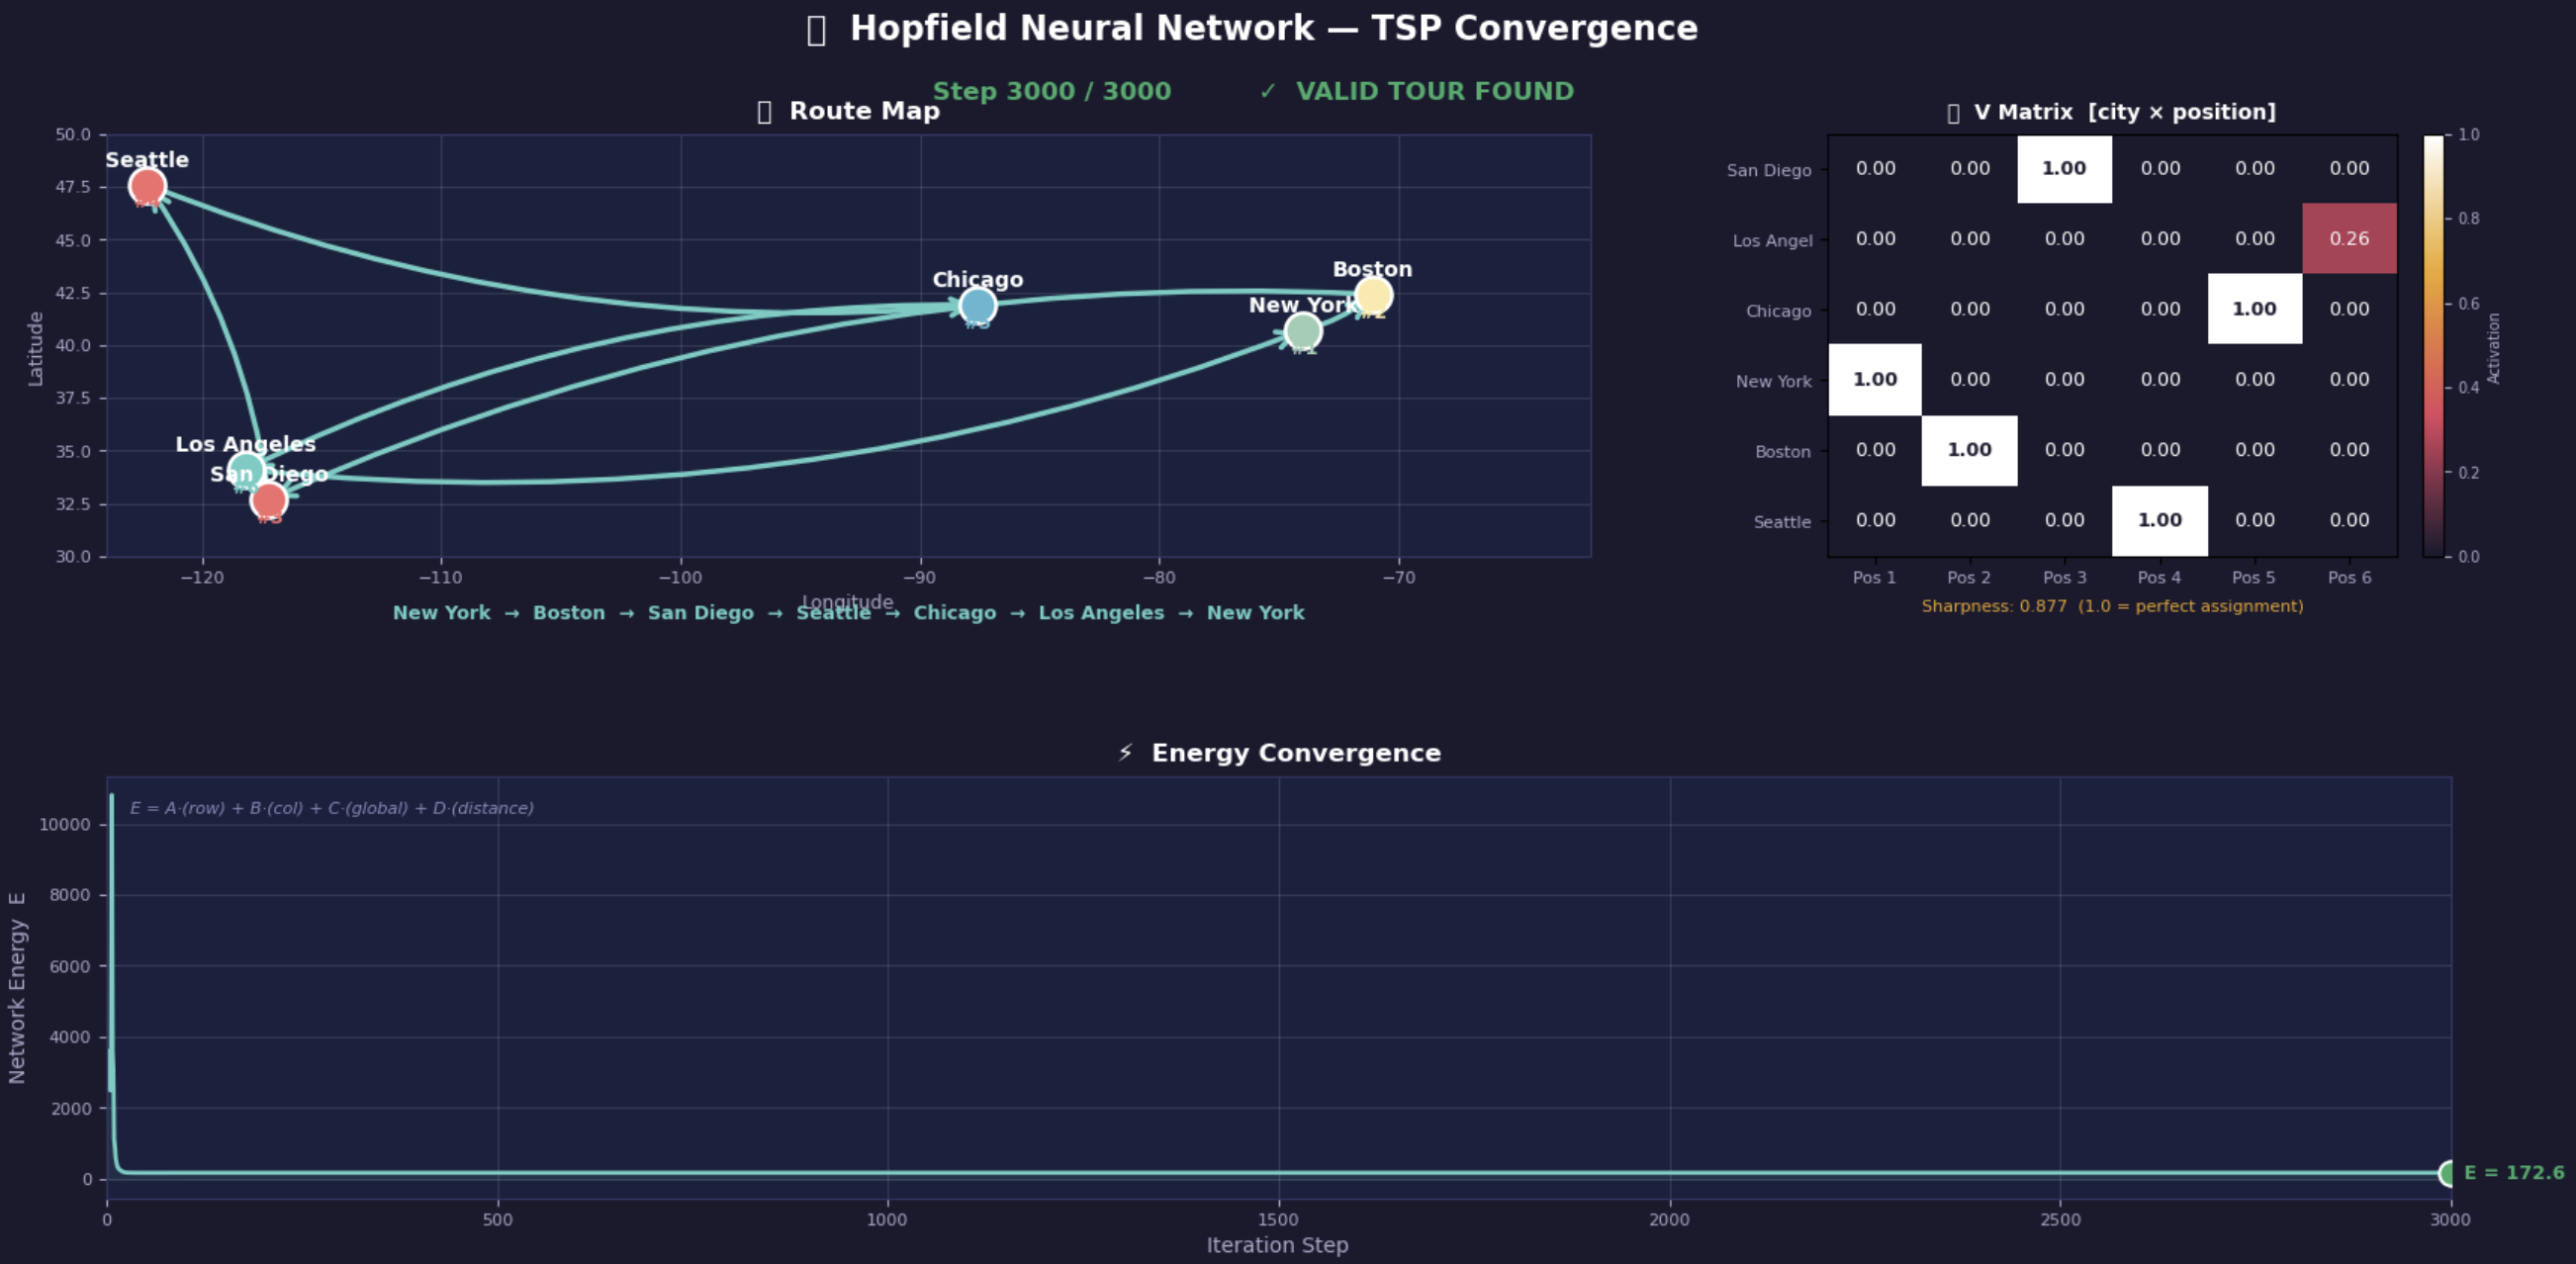
\includegraphics[width=0.6\textwidth]{Images/4.png}
        \end{center}
    \end{soln}
\end{prob}

\newpage

% --- Problem 5 ---
\begin{prob}[\textbf{(25 points) RNN for Periodic Function Modeling}]
    In this section, you will train an RNN for periodic function modeling. Assume we have a periodic function $f(t) : \R \to \R$ to model:

    \[  f(t) = \sin(at + b) \]

    We focus on modeling the sequence $\{f(t)\} = \{f(1), f(2)..., f(T - 1), f(T)\}$. Specifically, we aim to train a network to predict the next value of the function $f(t + 1)$ given the current value of the function $f(t)$ and previous hidden state $\h_{t-1}$. Thus, after training, if we have the initial value of function $f(1)$ and initial hidden state $\h_0$, we can iteratively generate the whole sequence $\{f(t)\}$. The following steps are used for sequence generation:

    \begin{enumerate}
        \item We use the current value of function $f(t)$ as input $\x_t \in \R^1$.
        \item Based on previous hidden state $\h_{t-1}$ and input $\x_t$, we can calculate the current hidden state $\h_t = \tanh(W_{xh} \x_t + W_{hh} \h_{t-1})$ and predict the output: $\y_t = W_{hy} \h_t \in \R^1$.
        \item We will use the current output $\y_t$ as next value of function $f(t + 1)$ and perform the above steps again.
    \end{enumerate}

    In the evaluation stage, if we have initial hidden state $\h_0$, initial value of function $f(1)$ and trained weight $W_{xh}$, $W_{hh}$, $W_{hy}$, we can utilize the above steps to generate the whole sequence $\{f(1), f(2), ..., f(T)\}$. Besides, if we have a partial sequence $\{f(1), f(2), ..., f(t - 1)\}$, we can also use the RNN to generate $\{f(t), f(t + 1), ..., f(T)\}$ to complete the sequence.

    In the training stage, we are given the sequence $\{f(1), f(2), ..., f(T)\}$. During training, we keep Step 1 and 2 above. Since we have the ground-truth for $f(t + 1)$ during training, we will compute the squared error $L_t = (f(t + 1) - \y_t)^2$ for all $t \in \{1, 2, ..., T - 1\}$ and optimize the average loss $L = \frac{1}{T - 1} \sum_{t=1}^{T - 1} L_t$. Note that $f(t + 1) - \y_t$ is actually a scalar operation since $\y_t \in \R^1$ can be regarded as a scalar.

    In PyTorch implementation, you only need to use \texttt{nn.RNNCell()} to perform $\h_t = \tanh(W_{xh} \x_t + W_{hh} \h_{t-1})$ and \texttt{nn.Linear()} to perform $\y_t = W_{hy} \h_t$. In the implementation, the input $\x_t$ and output $\y_t$ are both 1-dim vectors. The hidden state $\h_t \in \R^{100}$, which means there are 100 hidden neurons (i.e. hidden size = 100).

    \textbf{Note:}
    \begin{enumerate}
        \item In the description above, we ignore the bias terms, while in PyTorch implementation, both \newline\texttt{nn.RNNCell()} and \texttt{nn.Linear()} have bias terms at default. You can simply use the default setting of \texttt{nn.RNNCell()} and \texttt{nn.Linear()}.
    \end{enumerate}

    Download the skeleton code \texttt{hw5-periodic.ipynb} from the course website. Complete the skeleton code. In order to get full marks, your report should include:

    \begin{enumerate}
        \item Your code.
        \item Training loss curve.
        \item A figure of generated sequence.
    \end{enumerate}

    \textbf{Hint:} You may find the \href{https://pytorch.org/tutorials/beginner/deep_learning_60min_blitz.html}{official PyTorch tutorial} helpful before implementing the network.

    \begin{soln}
        Code and figure are attached at the end.
    \end{soln}
\end{prob}

\newpage

% --- Extra Credit ---
\begin{prob}[\textbf{(Extra Credit - 15 points) Char-RNN}]
    In section 2, you already obtain some experience with the forward procedure of RNN. In this section, you will train a special RNN called Char-RNN (i.e. Character RNN) on a language modeling task. Assume we have a character sequence $\{c_t\} = \{c_1, c_2..., c_{T - 1}, c_T \}$ where $c_t \in A$ and $A$ is the set of an alphabet (e.g. the character sequence can be $\{'n', 'e', 't', 'w', 'o', 'r', 'k'\}$, which will be used in the illustration below). We aim to train a network to predict the next character $c_{t+1}$ given current character $c_t$. Thus, after training, if we have initial character $c_1$, we can iteratively generate the whole sequence $\{c_t\}$:

    \begin{center}
        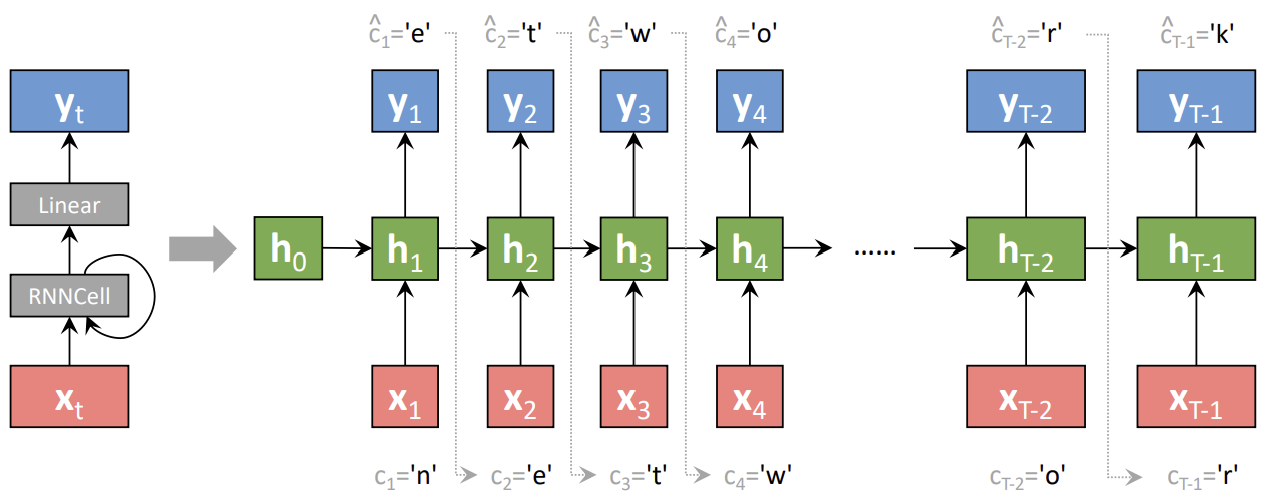
\includegraphics[width=0.5\textwidth]{Images/6.png}
    \end{center}

    The right part of the figure shows the “unrolled” version of the Char-RNN. Assume $|A| = K$, then we can represent the characters in alphabet $A$ into $K$ classes $\{0, 1..., K - 2, K - 1\}$. Then, we have the following steps for sequence generation:

    \begin{enumerate}
        \item We convert the input character $c_t$ into the one-hot encoding $\x_t \in \R^K$ of the class of the input character.
        \item Based on previous hidden state $\h_{t-1}$ and one-hot input $\x_t$, we can calculate the current hidden state $\h_t = \tanh(W_{xh} \x_t + W_{hh} \h_{t-1})$ and predict the output: $\y_t = W_{hy} \h_t$.
        \item Afterwards, we can use the softmax function to obtain the probability vector $\p_t = \text{Softmax}(\y_t) = \{p_0, ..., p_{K-1}\} \in \R^K$. Then, we will sample the class $\hat{k}$ from the probability vector $\p$ and find the corresponding character $\hat{c}_t$ as the predicted character. Note that here we do not use $\hat{k} = \arg \max_k p_k$ (i.e. the index with maximum probability) as prediction since it will reduce the diversity of the generated sequence.
        \item We will use the current predicted character $\hat{c}_t$ as next input character $c_{t+1}$ and perform the above steps again.
    \end{enumerate}

    In the evaluation stage, if we have initial hidden state $\h_0$, initial input character $c_1$ and trained weight $W_{xh}$, $W_{hh}$, $W_{hy}$, we can utilize the above steps to generate the whole sequence $\{c_1, c_2, ..., c_T\}$.

    In the training stage, we are given the sequence $\{c_1, c_2, ..., c_T\}$. During training, we keep Step 1 and 2 above and calculate the probability vector $\p_t$ in Step 3. Since we have the ground-truth for $c_{t+1}$ during training, we will compute the cross-entropy loss $L_t = \text{CrossEntropy}(\p_t, c_{t+1})$ for all $t \in \{1, 2, ..., T\}$ and optimize the average loss $L = \frac{1}{T} \sum_{t=1}^{T} L_t$.

    The left part of the figure shows the actual network in PyTorch implementation. You only need to use \texttt{nn.RNNCell()} to perform $\h_t = \tanh(W_{xh} \x_t + W_{hh} \h_{t-1})$ and \texttt{nn.Linear()} to perform $\y_t = W_{hy} \h_t$. In the implementation, we have the size of alphabet $K = 100$, which means one-hot input $\x_t$ and output $\y_t$ are both 100-dim vectors. The hidden state $\h_t \in \R^{100}$, which means there are 100 hidden neurons (i.e. hidden size = 100).

    \textbf{Note:} 
    \begin{enumerate}
        \item In the description above, we ignore the bias terms, while in PyTorch implementation, both \newline\texttt{nn.RNNCell()} and \texttt{nn.Linear()} have bias terms at default. You can simply use the default setting of \texttt{nn.RNNCell()} and \texttt{nn.Linear()}.
    \end{enumerate}

    \newpage

    Download the skeleton code \texttt{hw5-rnn.ipynb} from the course website. Complete the skeleton code. In order to get full marks, your report should include 

    \begin{enumerate}
        \item Your code
        \item Training loss curve
        \item A sample of generated sequence
    \end{enumerate}

    \textbf{Hint:} You may find the \href{https://pytorch.org/tutorials/beginner/deep_learning_60min_blitz.html}{official PyTorch tutorial} helpful before implementing the network.

    \begin{soln}
        Code and figure are attached at the end.
    \end{soln}
\end{prob}
\end{probset}
\end{document}